%%
%% InterruptLab (c) 2021-22 Christopher A. Bohn
%%
%% Licensed under the Apache License, Version 2.0 (the "License");
%% you may not use this file except in compliance with the License.
%% You may obtain a copy of the License at
%%     http://www.apache.org/licenses/LICENSE-2.0
%% Unless required by applicable law or agreed to in writing, software
%% distributed under the License is distributed on an "AS IS" BASIS,
%% WITHOUT WARRANTIES OR CONDITIONS OF ANY KIND, either express or implied.
%% See the License for the specific language governing permissions and
%% limitations under the License.
%%

%%
%% (c) 2021 Christopher A. Bohn
%%

\documentclass[12pt]{article}

\usepackage{fullpage}
\usepackage{fancyhdr}
\usepackage[procnames]{listings}
\usepackage{hyperref}
\usepackage{textcomp}
\usepackage{bold-extra}
\usepackage[dvipsnames]{xcolor}
\usepackage{etoolbox}


% Customize the semester (or quarter) and the course number

\newcommand{\courseterm}{Spring 2022}
\newcommand{\coursenumber}{CSCE 231}

% Customize how a typical lab will be managed;
% you can always use \renewcommand for one-offs

\newcommand{\runtimeenvironment}{your account on the \textit{csce.unl.edu} Linux server}
\newcommand{\filesource}{Canvas or {\footnotesize$\sim$}cse231 on \textit{csce.unl.edu}}
\newcommand{\filesubmission}{Canvas}

% These are placeholder commands and will be renewed in each lab

\newcommand{\labnumber}{}
\newcommand{\labname}{Lab \labnumber\ Assignment}
\newcommand{\shortlabname}{}
\newcommand{\duedate}{}

% Individual or team effort

\newcommand{\individualeffort}{This is an individual-effort project. You may discuss concepts and syntax with other students, but you may discuss solutions only with the professor and the TAs. Sharing code with or copying code from another student or the internet is prohibited.}
\newcommand{\teameffort}{This is a team-effort project. You may discuss concepts and syntax with other students, but you may discuss solutions only with your assigned partner(s), the professor, and the TAs. Sharing code with or copying code from a student who is not on your team, or from the internet, is prohibited.}
\newcommand{\freecollaboration}{In addition to the professor and the TAs, you may freely seek help on this assignment from other students.}
\newcommand{\collaborationrules}{}

% Do you care about software engineering?

\providebool{allowspaghetticode}

\setbool{allowspaghetticode}{false}

\newcommand{\softwareengineeringfrontmatter}{
    \ifboolexpe{not bool{allowspaghetticode}}{
        \section*{No Spaghetti Code Allowed}
        In the interest of keeping your code readable, you may \textit{not} use
        any \lstinline{goto} statements, nor may you use any \lstinline{break}
        statements to exit from a loop, nor may you have any functions
        \lstinline{return} from within a loop.
    }{}
}

\newcommand{\spaghetticodepenalties}[1]{
    \ifboolexpe{not bool{allowspaghetticode}}{
        \penaltyitem{1}{for each \lstinline{goto} statement, \lstinline{break}
            statement used to exit from a loop, or \lstinline{return} statement
            that occurs within a loop.}
    }{}
}

% You shouldn't need to customize these,
% but you can if you like

\lstset{language=C, tabsize=4, upquote=true, basicstyle=\ttfamily}
\newcommand{\function}[1]{\textbf{\lstinline{#1}}}
\setlength{\headsep}{0.7cm}
\hypersetup{colorlinks=true}

\newcommand{\startdocument}{
    \pagestyle{fancy}
    \fancyhf{}
    \lhead{\coursenumber}
    \chead{\ Lab \labnumber: \labname}
    \rhead{\courseterm}
    \cfoot{\shortlabname-\thepage}

	\begin{document}
	\title{\ Lab \labnumber}
	\author{\labname}
	\date{Due: \duedate}
	\maketitle

    \textit{\collaborationrules}
}

\newcommand{\rubricitem}[2]{\item[\underline{\hspace{1cm}} +#1] #2}
\newcommand{\bonusitem}[2]{\item[\underline{\hspace{1cm}} Bonus +#1] #2}
\newcommand{\penaltyitem}[2]{\item[\underline{\hspace{1cm}} -#1] #2}

%%
%% labs/common/semester.tex
%% (c) 2021-22 Christopher A. Bohn
%%
%% Licensed under the Apache License, Version 2.0 (the "License");
%% you may not use this file except in compliance with the License.
%% You may obtain a copy of the License at
%%     http://www.apache.org/licenses/LICENSE-2.0
%% Unless required by applicable law or agreed to in writing, software
%% distributed under the License is distributed on an "AS IS" BASIS,
%% WITHOUT WARRANTIES OR CONDITIONS OF ANY KIND, either express or implied.
%% See the License for the specific language governing permissions and
%% limitations under the License.
%%


% Customize the semester (or quarter) and the course number

\newcommand{\courseterm}{Fall 2022}
\newcommand{\coursenumber}{CSCE 231}

% Customize how a typical lab will be managed;
% you can always use \renewcommand for one-offs

\newcommand{\runtimeenvironment}{your account on the \textit{csce.unl.edu} Linux server}
\newcommand{\filesource}{Canvas or {\footnotesize$\sim$}cse231 on \textit{csce.unl.edu}}
\newcommand{\filesubmission}{Canvas}

% Customize for the I/O lab hardware

\newcommand{\developmentboard}{Arduino Nano}
%\newcommand{\serialprotocol}{SPI}
\newcommand{\serialprotocol}{I2C}
%\newcommand{\displaymodule}{MAX7219digits}
%\newcommand{\displaymodule}{MAX7219matrix}
\newcommand{\displaymodule}{LCD1602}

\setbool{usedisplayfont}{true}

\newcommand{\obtaininghardware}{
    The EE Shop has prepared ``class kits'' for CSCE 231; your class kit costs \$30.
    The EE Shop is located at 122 Scott Engineering Center and is open M-F 7am-4pm. You do not need an appointment.
    You may pay at the window with cash, with a personal check, or with your NCard.
    The EE shop does \textit{not} accept credit cards.
}

% Update to reflect the CS2 course(s) at your institute

\newcommand{\cstwo}{CSCE~156, RAIK~184H, or SOFT~161}

% Do you care about software engineering?

\setbool{allowspaghetticode}{false}

% Which assignments are you using this semester, and when are they due?

\newcommand{\pokerlabnumber}{1}
\newcommand{\pokerlabcollaboration}{
    Sections~\ref{sec:connecting}, \ref{sec:terminology}, \ref{sec:gettingstarted}, \ref{subsec:typesofpokerhands}, and~\ref{subsec:studythecode}: \freecollaboration
    Sections~\ref{sec:completingcard} and~\ref{subsec:completepoker}: \individualeffort
}
\newcommand{\pokerlabdue}{Week of August 29, before the start of your lab section}

\newcommand{\keyboardlabnumber}{2}
\newcommand{\keyboardlabcollaboration}{\individualeffort}
\newcommand{\keyboardlabdue}{Week of January 31, before the start of your lab section}

\newcommand{\pointerlabnumber}{3}
\newcommand{\pointerlabcollaboration}{\individualeffort}
\newcommand{\pointerlabdue}{Week of February 7, before the start of your lab section}

\newcommand{\integerlabnumber}{4}
\newcommand{\integerlabcollaboration}{\individualeffort}
\newcommand{\integerlabdue}{Week of February 14, before the start of your lab section}

\newcommand{\floatlabnumber}{5}
\newcommand{\floatlabcollaboration}{\individualeffort}
\newcommand{\floatlabdue}{soon}

\newcommand{\addressinglabnumber}{6}
\newcommand{\addressinglabcollaboration}{\individualeffort}
\newcommand{\addressinglabdue}{Week of February 28, before the start of your lab section}

%bomblab was 7
%attacklab was 8

\newcommand{\pollinglabnumber}{9}
\newcommand{\pollinglabcollaboration}{\individualeffort}
\newcommand{\pollinglabdue}{Week of April 11, before the start of your lab section}
\newcommand{\pollinglabenvironment}{your \developmentboard-based class hardware kit}

\newcommand{\ioprelabnumber}{\pollinglabnumber-prelab}
\newcommand{\ioprelabcollaboration}{\freecollaboration}
\newcommand{\ioprelabdue}{Before the start of your lab section on April 5 or 6}

\newcommand{\interruptlabnumber}{10}
\newcommand{\interruptlabcollaboration}{\individualeffort}
\newcommand{\interruptlabdue}{Week of April 18, before the start of your lab section}
\newcommand{\interruptlabenvironment}{your \developmentboard-based class hardware kit}

\newcommand{\capstonelab}{ComboLock}    % this will come into play when we generalize capstonelab
\newcommand{\capstonelabnumber}{11}
\newcommand{\capstonelabcollaboration}{\teameffort}
\newcommand{\capstonelabdue}{Week of May 2, Before the start of your lab section\footnote{See Piazza for the due dates of teams with students from different lab sections.}}
\newcommand{\capstonelabenvironment}{your \developmentboard-based class hardware kit}

\newcommand{\memorylabnumber}{12}
\newcommand{\memorylabcollaboration}{This is an individual-effort project. You may discuss the nature of memory technologies and of memory hierarchies with classmates, but you must draw your own conclusions.}
\newcommand{\memorylabdue}{Week of May 2, at the end of your lab section}
\newcommand{\memorylabenvironment}{your \developmentboard-based class hardware kit and your account on the \textit{csce.unl.edu} Linux server}

% Labs not used this semester

\newcommand{\concurrencylabnumber}{XX}
\newcommand{\concurrencylabcollaboration}{\individualeffort}
\newcommand{\concurrencylabdue}{not this semester}

\newcommand{\ssbcwarmupnumber}{XX}
\newcommand{\ssbcwarmupcollaboration}{\freecollaboration}
\newcommand{\ssbcwarmupdue}{not this semester}

\newcommand{\ssbcpollingnumber}{XX}
\newcommand{\ssbcpollingcollaboration}{\individualeffort}
\newcommand{\ssbcpollingdue}{not this semester}

\newcommand{\ssbcinterruptnumber}{XX}
\newcommand{\ssbcinterruptcollaboration}{\individualeffort}
\newcommand{\ssbcinterruptdue}{not this semester}

\usepackage{enumitem}
\usepackage{graphicx}
\usepackage{addfont}
\addfont{OT1}{d7seg}{\dviiseg}
% \addfont{OT1}{deseg}{\deseg}
\usepackage{subfig}
% \usepackage{wrapfig}
\usepackage{multicol}
% \usepackage{caption}
% \captionsetup{width=.8\linewidth}

% \lstset{language=c, numbers=left, showstringspaces=false,
%     moredelim = [s][\ttfamily]{/*}{*/} % I shouldn't need this parameter!
%     }



\renewcommand{\labnumber}{\interruptlabnumber}
\renewcommand{\labname}{Using Interrupt-Driven Input/Output}
\renewcommand{\shortlabname}{interrupt-driven i/o -- interruptlab}
\renewcommand{\collaborationrules}{\interruptlabcollaboration}
\renewcommand{\duedate}{\interruptlabdue}
\newcommand{\nano}{\developmentboard} % TODO: replace \nano with \developmentboard
\renewcommand{\runtimeenvironment}{\interruptlabenvironment}
\pagelayout
\begin{document}
\labidentifier

In this assignment, you will write code for \runtimeenvironment\ that will use
interrupts from external devices and from a timer to implement the ability to
convert numbers between radices.

\begin{figure}[h]
    \centering
    
\includegraphics[width=10cm]{MomMomMom}
    \caption{Interrupts. \tiny Image by 20th Century Fox Television}
\end{figure}

The instructions are written assuming you will edit the code in the Arduino IDE
and run it on \runtimeenvironment, constructed according to the pre-lab
instructions. If you wish, you may edit the code in a different environment;
however, our ability to provide support for problems with other IDEs is limited.

Please familiarize yourself with the entire assignment before beginning.
Section~\ref{sec:FunctionalSpecification} has the functional specification of
the system system you will develop. Section~\ref{sec:Constraints} describes
implementation constraints. Section~\ref{sec:Paradigm} relates interrupt-driven
I/O to event-driven programming (which you should have learned about in \cstwo).
Section~\ref{sec:GettingStarted} identifies code that you can reuse from PollingLab.
Section~\ref{sec:TimerInterrupts} will guide you through configuring a hardware
timer and responding to interrupts from that timer.
Section~\ref{sec:ExternalInterrupts} will guide you through registering and writing
interrupt service routines for external interrupts. Finally,
Sections~\ref{sec:ConversionTimeout} and \ref{sec:BuildingAndConverting} offers
suggestions for using your interrupt service routines to implement the system's
specifications.

\section*{Learning Objectives}

After successful completion of this assignment, students will be able to:
\begin{itemize}
\item Use tables from a datasheet to determine the bit vectors needed to
    configure I/O devices
\item Configure a hardware timer to generate interrupts
\item Register an interrupt service routine for an interrupt vector
\item Register an interrupt service routine using a higher abstraction
\item Use interrupt-driven I/O to realize simple requirements
\end{itemize}

\subsection*{Continuing Forward}

After completing PollingLab and InterruptLab, you will be ready for the Group
Project, in which you will implement a simple embedded system.

\section*{During Lab Time}

During your lab period, the TAs will demonstrate how to use tables from a
datasheet to construct bit vectors. During the remaining time, the TAs will be
available to answer questions.

\softwareengineeringfrontmatter

\section{Scenario}

Smoke wafts from Herb's soldering iron as he looks up when you approach.
Cleaning the iron's tip, he quotes: ``Somebody once said, `The three most
dangerous things in the world are a programmer with a soldering iron, a
hardware engineer with a software patch, and'{}'' -- he glances nervously in
Archie's direction -- ``{}`a user with an idea.'\footnote{Rick Cook, \textit{The
Wizardry Consulted}, 1995.}$^{\mathrm{,}}$\footnote{The notion of being wary of
programmers wielding screwdrivers or soldering irons long pre-dated this quote,
as there are apocryphal tales of people who found it easier to modify the
hardware to suit the software rather than the other way around.}'' Herb gets
straight to the point. ``We promised Archie that we'd be able to start using
the Cow Pi to build systems in a week. So far we've tested its input/output
functionality, but we still need to test its timer and also whether we can take
inputs without constantly polling the input devices. As before, we don't need
to do anything too fancy; let's try a number base conversion tool.''

\section{Number-Base Conversion Tool Specification} \label{sec:FunctionalSpecification}

\begin{enumerate}
\item The user shall be able to build a number.
    \begin{enumerate}
    \item \label{spec:initallyZero} The number being built shall initially hold the
        value 0.
    \item \label{spec:decimalExplained} When the \textbf{right switch} is
        toggled to the left, the conversion tool will use the decimal number
        base. When the user presses a button on the \textbf{matrix keypad} with
        a decimal numeral (\textit{0-9}) then the conversion tool shall take the
        appropriate action as specified below. Any other buttons on the keypad
        shall be ignored.
    \item \label{spec:hexadecimalExplained} When the \textbf{right switch} is
        toggled to the right, the conversion tool will use the hexadecimal
        number base. When the user presses a button on the \textbf{matrix
        keypad} then the conversion tool shall take the appropriate action as
        specified below. Buttons with decimal numerals (\textit{0-9}) or
         alphabetic letters (\textit{A-D}) shall be interpreted as having the
         corresponding hexadecimal numeral; the button with the octothorp (\#)
         shall be interpreted as having the hexadecimal numeral \textit{E}; and
         the button with the asterisk (*) shall be interpreted as having the
         hexadecimal numeral \textit{F}.
    \item \label{spec:displayZero} When the number being built holds the value 0,
        the \textbf{7-segment display module} shall display {\dviiseg 0} in the
        least-significant digit; no other digits shall be initially illuminated.
    \item \label{spec:BuildingValue} Whenever the user presses a button on the
        \textbf{matrix keypad}, the corresponding numeral shall be displayed in
        the least-significant position of the \textbf{7-segment display
        module}, and any digits already displayed shall increase in
        significance by one order of magnitude. For example, if {\dviiseg 234}
        is displayed and the user presses \texttt{5} then {\dviiseg 2345} shall
        be displayed. The numeral displayed shall follow the interpretations
        specified in requirements \ref{spec:decimalExplained} and
        \ref{spec:hexadecimalExplained}.
        \begin{enumerate}
        \item There shall be no noticeable lag in updating the display.
        \item \label{spec:printValueToConsole} The new value shall be printed
            to the Serial Monitor in decimal or hexadecimal, depending on the
            system's current number base.
        \end{enumerate}
    \item ``0x'' shall not be displayed as part of a hexadecimal value.
    \item A positive sign shall not be displayed as part of a positive value.
    \item If a negative decimal value is displayed, the negative sign shall
        be displayed immediately to the left of the most-significant digit
        being displayed. For example, {\dviiseg-456} is correctly
        displayed, but {\dviiseg -    456} is not correctly displayed.
    \item \label{spec:noLeadingZeroes} Except when the number being built holds
        the value 0 (see requirement~\ref{spec:displayZero}), leading 0s shall not
        be displayed. For example, {\dviiseg 782} is allowed, but {\dviiseg
        00000782} is not allowed.
    \item Whenever the user presses and then releases the \textbf{right
        pushbutton} at least 150ms later, the number being built shall reset to
        0, and the \textbf{7-segment display module} shall be cleared,
        \textit{except} that the least-significant digit shall display
        {\dviiseg 0} (this being the new number being built). \textit{The change
        shall take effect only when the user \underline{releases} the
        \textbf{right pushbutton}.}
    \item Whenever the user presses and then releases the \textbf{left
        pushbutton} at least 150ms later, the value being displayed shall be
        negated. \textit{The change shall take effect only when the user
        \underline{releases} the \textbf{left pushbutton}.}
        \begin{enumerate}
        \item In the decimal number base, the presence or absence of negative
            sign shall indicate whether or not a value is negative
        \item In the hexadecimal number base, 32-bit two's complement shall be
            used.
        \end{enumerate}
    \item In no case shall the tool allow the user to input a value too
        great to be displayed on the \textbf{7-segment display module}. If
        the user attempts to enter a value greater than $0x7FFF,FFFF$ in
        hexadecimal, less than $0x8000,0000$ in hexadecimal, greater than
        $99,999,999$ in decimal, or less than $-9,999,999$ in decimal, then the
        \textbf{7-segment display module} shall display {\dviiseg too big}.
        \begin{itemize}
        \item \textit{n.b.}, in a hexadecimal 32-bit negative integer, an
            \texttt{F} in the most-significant hex-digit might only be a sign
            extension; in this scenario, if the user inputs another hex-digit
            then it is still a valid number because it would not be less than
            $0x8000,0000$. \\ \\
            For example, adding another digit to the 32-bit integer
            $0xF865,4321$ would \textit{not} produce a too-great value because
            the 36-bit integer $0xF,8654,3210 = -2,041,302,512_{10}$, and the
            32-bit integer $0x8654,3210 = -2,041,302,512_{10}$. Because
            $0x8000,0000 = -2,147,483,648_{10} \leq -2,041,302,512_{10}$, adding
            the \texttt{0} digit did not produce a ``too big'' value. \\ \\
            On the other hand, adding another digit to the 32-bit integer
            $0xF765,4321$ \textit{would} produce a too-great value because the
            36-bit integer $0xF,7654,3210 = -2,309,737,968_{10}$, but the 32-bit
            integer $0x8654,3210 = 1,985,229,328_{10}$. Because
            $0x8000,0000 = -2,147,483,648_{10} > -2,309,737,968_{10}$, adding
            the \texttt{0} digit did produce a ``too big'' value.
        \end{itemize}
    \item Nothing shall be printed on the Serial Monitor when the system is in
        building mode.
    \end{enumerate}
\item The user shall be able to see the number converted to a different number
    base.
    \begin{enumerate}
    \item Whenever the user presses double-clicks the \textbf{left pushbutton},
        the \textbf{7-segment display module} shall display the number in the
        opposite number base. \textbf{A \textit{double-click} is defined as
        pressing the button and releasing it no more than 150ms later, and
        pressing it again no later than 500ms after that.}
        \begin{enumerate}
            \item If the \textbf{right switch} is toggled to the left, then the
                decimal number shall be displayed as the equivalent hexadecimal
                number.
            \item If the \textbf{right switch} is toggled to the right, then the
                hexadecimal number shall be displayed as the equivalent decimal
                number.
            \item If the value is too great to be displayed in the new number
                base, then {\dviiseg error} shall be displayed.
        \end{enumerate}
    \item The conversion shall take place immediately after the
        \textbf{left pushbutton} is double-clicked.
    \item If the \textbf{left switch} is toggled to the left, then exactly 20
        seconds after the \textbf{left pushbutton} is double-clicked, the number
        shall be displayed in its original number base.
    \item If the \textbf{left switch} is toggled to the right, then exactly 7.5
        seconds after the \textbf{left pushbutton} is double-clicked, the number
        shall be displayed in its original number base.
    \item If {\dviiseg error} is displayed due to the value being too great to
        be displayed in the new number base, then after 7.5~seconds or
        20~seconds (as appropriate) has elapsed, {\dviiseg error} shall no
        longer be displayed, and the number shall be displayed in its original
        number base.
    \item While the converted number is being displayed, the \textbf{external
        LED} shall be illuminated. When the number is being displayed in its
        original number base, the \textbf{external LED} shall not be
        illuminated.
    \item If the \textbf{left pushbutton} is double-clicked, then releasing the
        \textbf{left pushbtton} shall not cause the number to be negated.
    \end{enumerate}
\item If the user changes the position of the \textbf{right switch} while the
    number is a value other than 0, the system's behavior is unspecified.
\item If the user changes the position of the \textbf{left switch} while the
    coverted number is being displayed, the system's behavior is unspecified.
\item If the user presses a key on the keypad or one of the pushbuttons while
    the converted number is being displayed, the system's behavior is
    unspecified.
    \begin{itemize}
    \item After the number in its original number base is again displayed, the
    system's behavior is as specified above.
    \end{itemize}
\end{enumerate}

\section{Constraints}\label{sec:Constraints}

You may continue to use the memory-mapped I/O registers, or you can use
functions provided by the Arduino core read from and write to pins.

You may re-use code from the previous lab, or you can rewrite the necessary
code using functions, macros, types, or constants that are part of the Arduino
core;\footnote{\url{https://www.arduino.cc/reference/en/}} functions, macros,
types, or constants of
avr-libc;\footnote{\url{https://www.nongnu.org/avr-libc/user-manual/index.html}}
or one of Arduino's standard
libraries.\footnote{\url{https://www.arduino.cc/reference/en/libraries/} The
standard libraries are those under the heading, ``Standard Libraries.''} You
may \textit{not} use a third-party library, not even one that the Arduino
Libraries reference page links to (if it isn't among those available in the
Arudino IDE's ``Sketch'' $\rightarrow$ ``Include Library'' menu under
``Arduino libraries'' then you may not use it).

You may \textit{not} poll the matrix keypad nor the pushbuttons to determine
if they have been pressed. You must use interrupts to determine if a key or
button has been pressed. Once a press has been detected, you may scan the
matrix keypad or read the pushbuttons to determine which key or button has
been pressed.

You may poll the switches to determine if either's position has changed;
however, the specification has been written such that your code should only
need to occasionally check the switches' positions rather than polling them for
changes.

While it is possible to configure the SPI hardware to generate an interrupt
after the content of the SPI Data Register is transmitted, you may use your
\function{displayData()} function that polls the \texttt{SPIF} bit.

While you may use \function{millis()} for debouncing, you may \textit{not} use
\function{millis()} nor \function{micros()} to determine when a converted number
should return to being displayed in its original number base. You must use an
interrupt from the ATmega328P's Timer1 or Timer2 to determine when a converted
number should reutrn to being displayed in its original number base.

While it is typically okay to have code in \function{loop()} while also using
interrupts, you may \textit{not} have any code in the \function{loop()}
function for this assignment. You also may not introduce an infinite loop
elsewhere in your program. While you typically want to keep your interrupt
service routines (ISRs) as short as possible, you may (indeed, you must) have
all of your logic in your interrupt service routines (or functions called by
your ISRs) for this assignment.

Do \textit{not} edit \textit{cowpi.h}; all of your code must go in
\textit{InterruptLab.ino}.

\section{A Different but Familiar Programming Paradigm} \label{sec:Paradigm}

Most of the code you wrote in the earlier lab assignments for this courses used
imperative programming: you, the programmer, had full control over changes to
the program state. In PollingLab, you stretched this model to something
resembling shared-memory concurrent programming: you still had full control
over changes to the program state of your program's flow of control, but your
program periodically read variables (memory-mapped input registers) that coul
changed by another flow of control (the physical world).

In this lab assignment, you will write code that reacts to things happening in
the physical world; none of your code will run except in reaction to interrupts.
Conceptually, this isn't very different from event-driven programming that you
learned in \cstwo. While configuring the hardware timer is a little more complex
than configuring a GUI framework's timer, handling a timer interrupt is very
much like writing an \function{onTimeout()} event handler. Similarly, handling
a change in a pushbutton's position is very much like writing an
\function{onMouseClick} event handler. Your code is not focused on \textit{when}
the button is pressed or released, nor even on \textit{detecting} that a button
has been pressed or released; it is focused solely on \textit{what should happen}
when the button is pressed or released.

\section{Getting Started} \label{sec:GettingStarted}

Copy code from your \textit{PollingLab.ino} into \textit{InterruptLab.ino} that
you think may be useful, such as \function{displayData()}, the address
assignments to \lstinline{ioPorts} and \lstinline{spi}, and assorted global
arrays. You will want to keep your code for scanning the keypad handy, as you
will be able to reuse most of it with only a few modifications. You will also
want to keep your code for building numbers handy, though it will require
several changes.

If you did not successfully implement \function{displayData()} during
PollingLab, you may have \function{displayData()} simply call
\function{cowpi_sendDataToMax7219(address, value)}. If you did not successfully
implement \function{getKeypressed()} during PollingLab, you may have
\function{handleKeypress()} call \function{cowpi_getKeypress()} (note that
\function{cowpi_getKeypress()}) does not take care of switch debouncing, and it
returns the character corresponding to the symbol on the key that was pressed,
not the numeric value specified by this assignment.)

If you need to rewrite any other code from the previous lab, you may do so
without explicitly using the memory-mapped I/O registers. You may instead use
\function{digitalRead()}\footnote{\url{https://www.arduino.cc/reference/en/language/functions/digital-io/digitalread/}}
and \function{digitalWrite()}\footnote{\url{https://www.arduino.cc/reference/en/language/functions/digital-io/digitalwrite/}}
to perform input and output on specific pins.

\section{Detecting Time}\label{sec:TimerInterrupts}

You must use timer interrupts from either Timer1 or Timer2 as part of your
implementation of the conversion timeout. Without using an external clock source,
you won't be able to configure an interrupt to occur every 20 seconds, or even
every 7.5 seconds. Since we will not use an external clock source, you will need
to use timer interrupts along with other logic.

\subsection{Preparation}

Design your logic and determine how often you need a timer interrupt to make it
work. For example, the \nano's pseudorealtime clock relies on an interrupt from
Timer0 every 1.024µs and advances the millisecond counter after 1,000 of these
interrupts have occurred. The pseudorealtime clock uses an overflow-based timer
interrupt to arrive at an approximation of milliseconds. The conversion tool's
specification calls for the converted number to display for exactly 7.5 seconds
or exactly 20 seconds (depending on the switch position) before the original
number is displayed again. To achieve exactness, you will use a comparison-based
timer.

You can then determine the parameters for the timer using
this equation:
\[
16,000,000 \frac{\mathrm{cycles}}{\mathrm{second}} =
    comparison\_value \frac{\mathrm{beats}}{\mathrm{interrupt}} \times
    prescaler \frac{\mathrm{cycles}}{\mathrm{beat}} \times
    interrupt\_frequency \frac{\mathrm{interrupts}}{\mathrm{second}}
\]
or, equivalently:
\[
    comparison\_value \frac{\mathrm{beats}}{\mathrm{interrupt}} \times
    prescaler \frac{\mathrm{cycles}}{\mathrm{beat}} =
    16,000,000 \frac{\mathrm{cycles}}{\mathrm{second}} \times
    interrupt\_period \frac{\mathrm{seconds}}{\mathrm{interrupt}}
\]
where:
    \begin{description}
    \item [16,000,000 Hz] is the clock frequency (the inverse of the clock
        period).
    \item [comparison\_value] is a number you will place in one of the
        timer's \texttt{compare} registers for a comparison-based timer
        interrupt. This can be any possible value of an unsigned 16-bit integer
        for Timer1, or any possible value of an unsigned 8-bit integer for
        Timer2.
    \item [prescaler] is a multiplier applied to the clock period to adjust the
        time between counter increments (``beats''). Possible values are 1, 8,
        64, 256, and 1024 for Timer1, or 1, 8, 32, 64, 128, 256, and 1024 for
        Timer2.
    \item [interrupt\_frequency] is how often you want a timer interrupt (the
        inverse of the interrupt period).
    \item [interrupt\_period] is the time between timer interrupts (the
        inverse of the interrupt frequency).
    \end{description}

You may have to iterate on your design until you arrive at one that works with
the constraints of that equation's terms for whichever timer you choose to use.

The Waveform Generation Mode you will use is \textit{CTC} (Clear Timer on
Compare) with the ``TOP'' value set by the \texttt{OCRnA} (\textit{compareA})
register, where $n$ is the Timer number. Use Figure~\ref{fig:Timer1WGM} (for
Timer1) or Figure~\ref{fig:Timer2WGM} (for Timer2) to select the appropriate
\texttt{WGM13}~\texttt{WGM12}~\texttt{WGM11}~\texttt{WGM10} or
\texttt{WGM22}~\texttt{WGM21}~\texttt{WGM20} bits.

Based on the prescaler you chose for the above equation, select the appropriate
\texttt{CS12}~\texttt{CS11}~\texttt{CS10} or
\texttt{CS22}~\texttt{CS20}~\texttt{CS20} bits from Figure~\ref{fig:Timer1CS}
(for Timer1) or Figure~\ref{fig:Timer2CS} (for Timer2).

\begin{figure}[p]
    \centering
    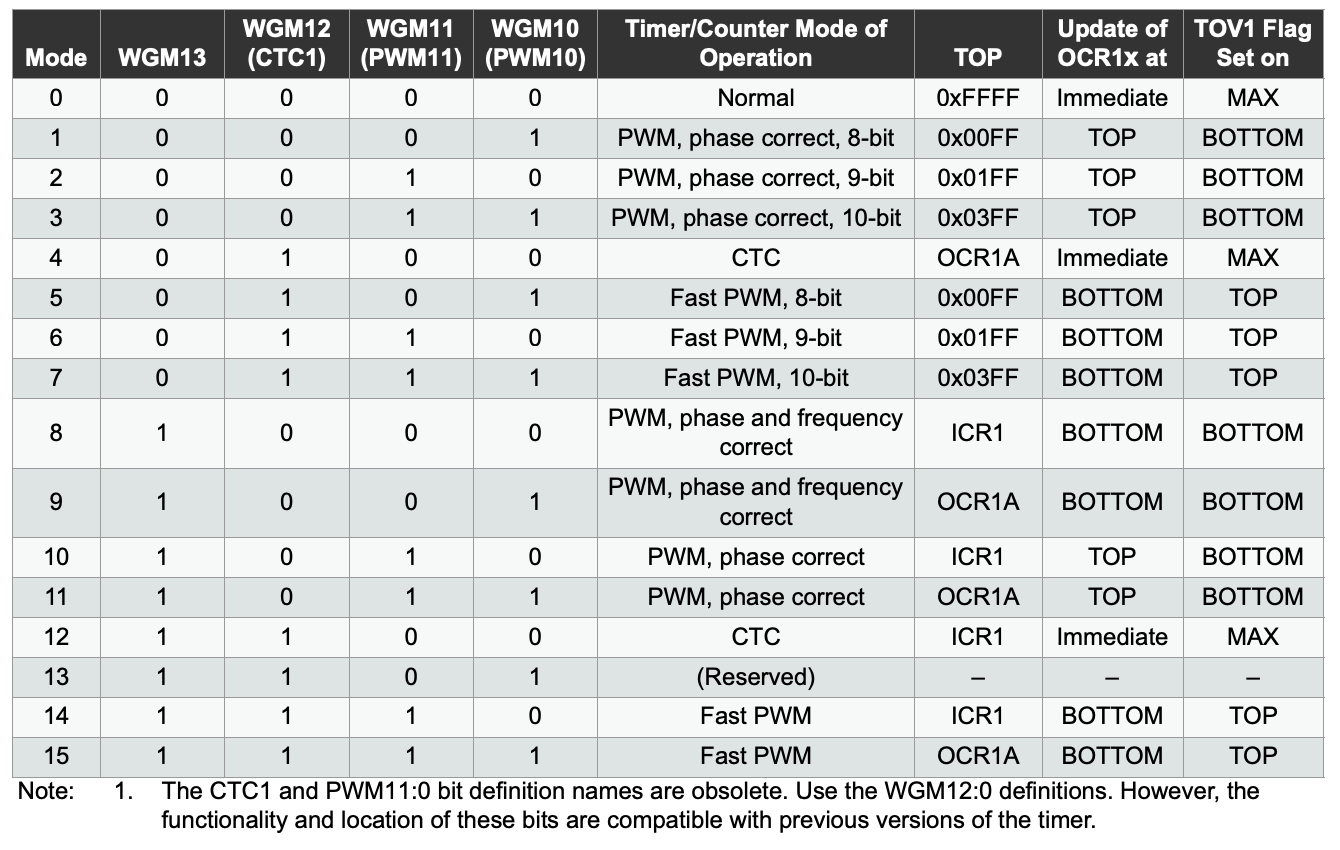
\includegraphics[width=15cm]{WGM-Timer1}
    \caption{Waveform Generation Mode Bit Description for Timer1. \tiny Copied from ATmega382P Data Sheet, Table~15-5 \label{fig:Timer1WGM}}
\end{figure}

\begin{figure}[p]
    \centering
    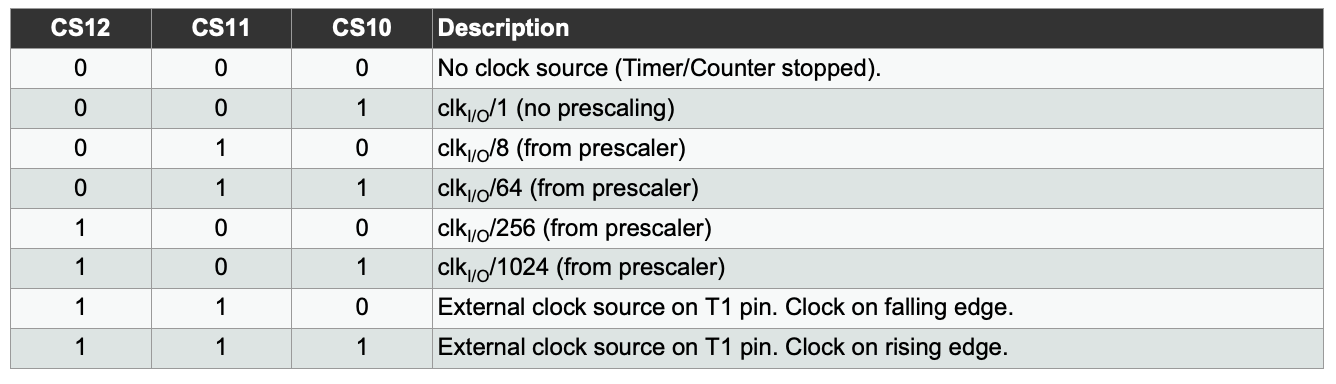
\includegraphics[width=15cm]{CS-Timer1}
    \caption{Clock Select Bit Description for Timer1. \tiny Copied from ATmega382P Data Sheet, Table~15-6 \label{fig:Timer1CS}}
\end{figure}

\begin{figure}[p]
    \centering
    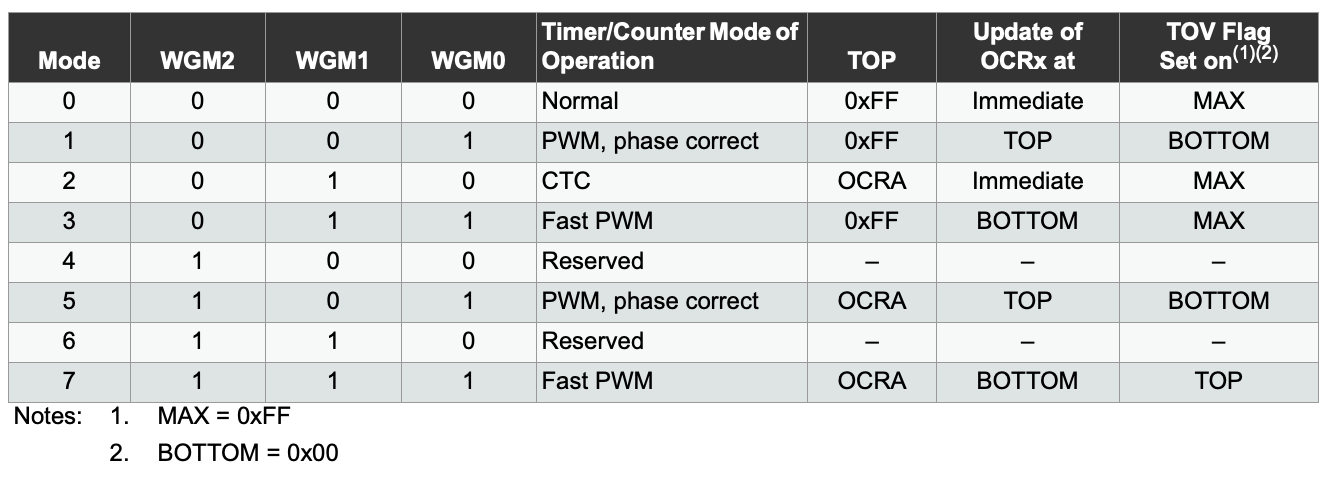
\includegraphics[width=15cm]{WGM-Timer2}
    \caption{Waveform Generation Mode Bit Description for Timer2. \texttt{WGM22}, \texttt{WGM21}, and \texttt{WGM20} are incorrectly shown here as \texttt{WGM2}, \texttt{WGM1}, and \texttt{WGM0}. \texttt{OCR2A} is incorrectly shown here as \texttt{OCRA}. \tiny Copied from ATmega382P Data Sheet, Table~17-8 \label{fig:Timer2WGM}}
\end{figure}

\begin{figure}[p]
    \centering
    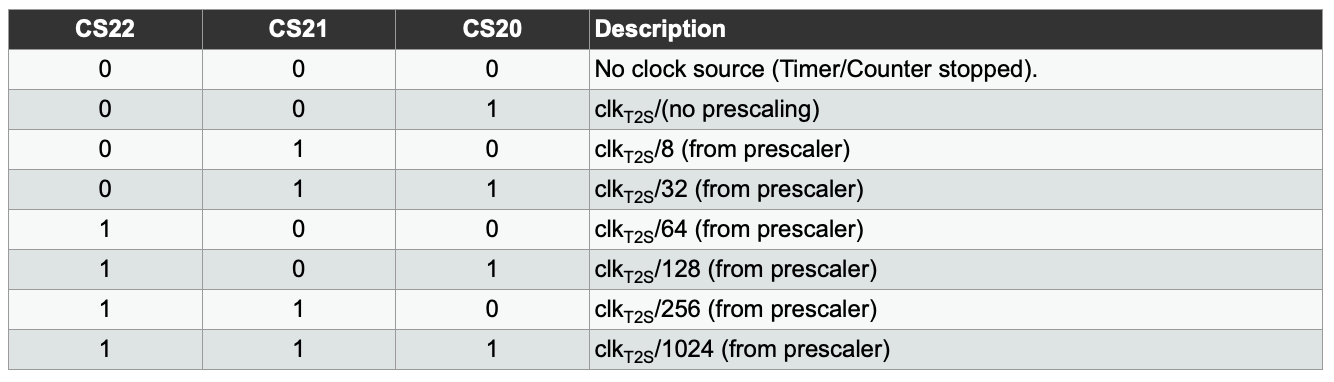
\includegraphics[width=15cm]{CS-Timer2}
    \caption{Clock Select Bit Description for Timer2. \tiny Copied from ATmega382P Data Sheet, Table~17-9 \label{fig:Timer2CS}}
\end{figure}

\subsection{Setup}

You may configure the timer using either memory-mapped I/O or using macros
provided by AVR-libc.\footnote{AVR-libc provides macros named after the I/O
registers that allow you to read from and write to these registers as though
they were ordinary variables.}

In the \function{setupTimer()} function:

\subsubsection{If using memory-mapped I/O}

Configure the timer:
\begin{itemize}
\item If you will use Timer1, remove the comment marks and elipses for the
    \lstinline{timer1} global variable. Assign to \lstinline{timer1} the address
    \lstinline{(cowpi_timerRegisters16bit *)(cowpi_IObase + 0x60)}. You can
    delete the commented-out assignment to \lstinline{timer2}.
\item If you will use Timer2, remove the comment marks and elipses for the
    \lstinline{timer2} global variable. Assign to \lstinline{timer2} the address
    \lstinline{(cowpi_timerRegisters8bit *)(cowpi_IObase + 0x90)}. You can delete
    the commented-out assignment to \lstinline{timer1}.
\item Use \lstinline{timer1}'s or \lstinline{timer2}'s \lstinline{control} field to
    set the \texttt{WGM} and \texttt{CS} bits in the timer's control registers.
    \begin{itemize}
    \item Use Tables~\ref{table:Timer1Registers} and \ref{table:Timer1Control}
        (for Timer1) or Tables~\ref{table:Timer2Registers} and
        \ref{table:Timer2Control} (for Timer2) to determine where the
        \texttt{WGM} and \texttt{CS} bits are located in the control registers.
    \end{itemize}
\item Subtract one from your computed $comparison\_value$, and assign the
    resulting value to \lstinline{timer1}'s or \lstinline{timer2}'s
    \lstinline{compareA} field.\footnote{\label{note:subtractOne} You will
    subtract one because counting the integer values in the range
    $0\dots(comparison\_value-1)$ will count the $comparison\_value$ beats
    between timer interrupts. Realistically, on the human-scale, you probably
    won't notice the difference.}
\end{itemize}

Enable the comparison-based timer interrupt:
\begin{itemize}
\item Create a pointer to a \lstinline{volatile uint8_t} and assign to it the
    address \lstinline{cowpi_IObase + 0x4E}.
\item Treat the pointer as an array, and use the timer number (1 or 2) for the
    index when making an assignment.
\end{itemize}

You want to place a 1 in the \texttt{OCIEnA} bit (where $n$ is the timer
number); use Figure~\ref{fig:TimerInterruptRegisters} to determine the
appropriate bit to set.

\subsubsection{If using AVR-libc macros}

Configure the timer:
\begin{itemize}
\item If you will use Timer1, use Table~\ref{table:Timer1Control} to determine
    where the \texttt{WGM} and \texttt{CS} bits are located in the control
    registers. Make the relevant assignments to \lstinline{TCCR1A} and/or
    \lstinline{TCCR1B}.
\item If you will use Timer2, use Table~\ref{table:Timer2Control} to determine
    where the \texttt{WGM} and \texttt{CS} bits are located in the control
    registers. Make the relevant assignments to \lstinline{TCCR2A} and/or
    \lstinline{TCCR2B}.
\item Subtract one from your computed $comparison\_value$, and assign the
    resulting value to to OCR1A (Timer1) or OCR2A (Timer2).\textsuperscript{\ref{note:subtractOne}}
\end{itemize}

Enable the comparison-based timer interrupt:
\begin{itemize}
\item Make an assignment to \texttt{TIMSK1} for Timer1, or to \texttt{TIMSK2}
    for Timer2.
\end{itemize}

You want to place a 1 in the \texttt{OCIEnA} bit (where $n$ is the timer
number); use Figure~\ref{fig:TimerInterruptRegisters} to determine the
appropriate bit to set.

\begin{table}[p]
    \centering \small
    \begin{tabular}{|r||c|c|c|c||}
        \hline
        Bits                & \textbf{31..24}   & \textbf{23..16}   & \textbf{15..8}    & \textbf{7..0}     \\ \cline{2-5}
        \textbf{control}    & \textit{reserved} & \texttt{TCCR1C}   & \texttt{TCCR1B}   & \texttt{TCCR1A}   \\
        \textbf{counter}    & \multicolumn{2}{c|}{}                 & \multicolumn{2}{c||}{\texttt{TCNT1}}  \\
        \textbf{capture}    & \multicolumn{2}{c|}{}                 & \multicolumn{2}{c||}{\texttt{ICR1}}   \\
        \textbf{compareA}   & \multicolumn{2}{c|}{}                 & \multicolumn{2}{c||}{\texttt{OCR1A}}  \\
        \textbf{compareB}   & \multicolumn{2}{c|}{}                 & \multicolumn{2}{c||}{\texttt{OCR1B}}  \\ \hline
    \end{tabular}
    \caption{Relationship of \lstinline{cowpi_timerRegisters16bit} fields to Timer1's registers. \tiny Adapted from ATmega382P Data Sheet, §15.11. \label{table:Timer1Registers}}
\end{table}

\begin{table}[p]
    \centering \small
    \begin{tabular}{|r||c|c|c|c|c|c|c|c||}
        \hline
        Bit             & \textbf{7}        & \textbf{6}        & \textbf{5}        & \textbf{4}        & \textbf{3}        & \textbf{2}    & \textbf{1}        & \textbf{0}        \\ \cline{2-9}
        \textbf{TCCR1C} & \texttt{FOC1A}    & \texttt{FOC1B}    & -                 & -                 & -                 & -             & -                 & -                 \\
        \textbf{TCCR1B} & \texttt{ICNC1}    & \texttt{ICES1}    & -                 & \texttt{WGM13}    & \texttt{WGM12}    & \texttt{CS12} & \texttt{CS11}     & \texttt{CS10}     \\
        \textbf{TCCR1A} & \texttt{COM1A1}   & \texttt{COM1A0}   & \texttt{COM1BA1}  & \texttt{COM1B0}   & -                 & -             & \texttt{WGM11}    & \texttt{WGM10}    \\ \hline
    \end{tabular}
    \caption{Timer1's control registers. \tiny Adapted from ATmega382P Data Sheet, §15.11. \label{table:Timer1Control}}
\end{table}

\begin{table}[p]
    \centering \small
    \begin{tabular}{|r||c|c||}
        \hline
        Bits                & \textbf{15..8}    & \textbf{7..0}     \\ \cline{2-3}
        \textbf{control}    & \texttt{TCCR2B}   & \texttt{TCCR2A}   \\
        \textbf{counter}    &                   & \texttt{TCNT2}    \\
        \textbf{compareA}   &                   & \texttt{OCR2A}    \\
        \textbf{compareB}   &                   & \texttt{OCR2B}    \\ \hline
    \end{tabular}
    \caption{Relationship of \lstinline{cowpi_timerRegisters8bit} fields to Timer2's registers. \tiny Adapted from ATmega382P Data Sheet, §17.11. \label{table:Timer2Registers}}
\end{table}

\begin{table}[p]
    \centering \small
    \begin{tabular}{|r||c|c|c|c|c|c|c|c||}
        \hline
        Bit             & \textbf{7}        & \textbf{6}        & \textbf{5}        & \textbf{4}        & \textbf{3}        & \textbf{2}    & \textbf{1}        & \textbf{0}        \\ \cline{2-9}
        \textbf{TCCR2B} & \texttt{FOC2A}    & \texttt{FOC2B}    & -                 & -                 & \texttt{WGM22}    & \texttt{CS22} & \texttt{CS21}     & \texttt{CS20}     \\
        \textbf{TCCR2A} & \texttt{COM2A1}   & \texttt{COM2A0}   & \texttt{COM2BA1}  & \texttt{COM2B0}   & -                 & -             & \texttt{WGM21}    & \texttt{WGM20}    \\ \hline
    \end{tabular}
    \caption{Timer2's control registers. \tiny Adapted from ATmega382P Data Sheet, §17.11. \label{table:Timer2Control}}
\end{table}

\begin{figure}[p]
    \centering
    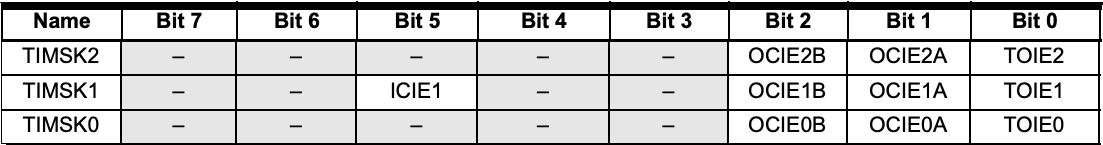
\includegraphics[width=15cm]{TimerInterruptRegisters}
    \caption{Timer interrupt registers. \tiny Cropped from ATmega382P Data Sheet, §30 \label{fig:TimerInterruptRegisters}}
\end{figure}


\subsection{Interrupt Service Routine}

Because the Arduino core does not provide a more convenient way to create an
interrupt service routine (ISR) for timer interrupts, you will use AVR-libc's
\function{ISR}\footnote{\url{https://www.nongnu.org/avr-libc/user-manual/group__avr__interrupts.html}}
macro.

In \textit{InterruptLab.ino}, outside of any other function, write this code that looks like a function:

\begin{lstlisting}
ISR(vector) {
    ...
}
\end{lstlisting}

where $vector$ is \lstinline{TIMER1_COMPA_vect} for Timer1 or
\lstinline{TIMER2_COMPA_vect} for Timer2. Replace ``\dots'' with the code that
should execute whenever the timer interrupt occurs.

For now, simply place a \function{println} statement in your ISR code to verify
that you have the timing correct. Later you will replace the \function{println}
statement with the code you need for your logic.

\textbf{NOTE} Any global variables used by your ISR should be declared as \lstinline{volatile}.

\textbf{NOTE} If you ever need to ``reset'' a timer's count back to 0, you can
simply write 0 to \lstinline{timer1}/\lstinline{timer2}'s' \lstinline{counter}
field or to \texttt{TCNT1}/\texttt{TCNT2}.

\section{Detecting Key and Button Presses}\label{sec:ExternalInterrupts}

For external interrupts, the Arduino core has abstracted-away all of the
configuration details.\footnote{\url{https://www.arduino.cc/reference/en/language/functions/external-interrupts/attachinterrupt/}}
Placing a call to
\begin{lstlisting}
attachInterrupt(digitalPinToInterrupt(pinNumber), isrName, mode);
\end{lstlisting}
will configure all of the necessary registers to call the function
\function{isrName()} whenever the input value on the pin \textit{pinNumber}
satisfies the \textit{mode}.

\subsection{Setup}

The two functions that we recommend be called in response to a keypress on the
matrix keypad and in response to pressing or releasing a pushbutton,
\function{handleKeypress()} and \function{handleButtonAction()}, are already stubbed
in \textit{InterruptLab.ino}.

Recall that the NAND output for the matrix keypad columns provides input to
\texttt{D3} and that the NAND output for the pushbuttons provides input to
\texttt{D2}. Decide on the \textit{mode} for the external interrupts:
    \begin{description}
    \item [LOW] to trigger the interrupt whenever the pin is low
    \item [RISING] to trigger the interrupt whenever the pin goes from low to
        high
    \item [FALLING] to trigger the interrupt whenever the pin goes from high to
        low
    \item [CHANGE] to trigger the interrupt whenever the pin rises or falls
    \end{description}
Because we did not provide a hardware solution to switch bounce, you can expect
the pin input to both rise and fall a few times when a button or key is
pressed and again when it is released -- but there is no guarantee that
bouncing will occur. For this reason we recommend:
    \begin{itemize}
    \item Use the \lstinline{CHANGE} mode, combined with software debouncing,
        and use a variable to keep track of whether a key or button has been
        pressed (toggle this variable whenever an interrupt occurs, and take
        action based on whether a key or button has been pressed or released).
    \item The software debouncing will look similar to what you used in
        PollingLab except that it only needs to be a few milliseconds instead
        of 500. Since we are not polling the buttons and keypad to detect
        presses, we do not need to worry about the button or key being held for
        several dozen milliseconds being interpretted as multiple presses.
        \begin{itemize}
        \item I very strongly advise against using \function{delay()} for
            software debouncing:
        \item As described in the PollingLab assignment sheet,
            \function{delay()} will leave your system unresponsive to anything
            except interrupts.
        \item Including \function{delay()} calls in an interrupt handler is
            particularly ill-advised since you may find yourself in a situation
            in which you need to disable interrupts in the interrupt handler
            and then re-enable interrupts before exiting the interrupt handler.
            (I do not expect this to happen in this assignment, but I've been
            wrong before.) The \function{delay()} function will never exit,
            blocking forever, if interrupts are disabled.
        \end{itemize}
    \end{itemize}
If you arrive at a different solution that works (including using more than the
two stubbed ISRs), you may use your solution.

In the \function{setup()} function, register your ISR functions for the external
interrupts:
\begin{lstlisting}
attachInterrupt(digitalPinToInterrupt(2), handleButtonAction, CHANGE);
attachInterrupt(digitalPinToInterrupt(3), handleKeypress, CHANGE);
\end{lstlisting}
(Here I assumed you would use the CHANGE mode. If you use a different mode,
replace CHANGE with the mode you chose. Similarly, if you use more than the two
stubbed ISRs, register those ISRs, too.)

\subsection{Handling Button Actions}

Your pushbutton handler (\function{handleButtonAction()}) needs to
determine which button was pressed or released, and whether it was pressed or
released -- this can be as simple as keeping track of each button's position and
calling \lstinline{digitalRead(8)} and
\lstinline{digitalRead(9)}.\footnote{Another way to determine if a button was
pressed or released is to use separate ISRs for \lstinline{RISING} and
\lstinline{FALLING}; however, you will still need to determine \textit{which}
button rose or fell, and whether it was due to the button being manipulated or
due to switch bounce.} Don't forget to include software debouncing. If
insufficient time (a few milliseconds) has passed since the last time the button
handler was invoked, you can simply exit the handler function under the
assumption that switch bounce is generating erroneous interrupts.

\textbf{NOTE} Any global variables used by your ISR should be declared as
\lstinline{volatile}.

For now, place a \function{println} statement in your ISR code indicating the
pushbuttons' positions to confirm that you are correctly detecting which button
has been pressed or released and whether it was pressed or released.

\subsection{Handling Key Presses}

Your keypad handler (\function{handleKeypress}) needs to determine which key was
pressed -- you can reuse your code from PollingLab that scans the keypad with
minimal changes. One such change is that you don't need to \lstinline{return} a
value. If insufficient time (a few milliseconds) has passed since the last time
the keypad handler was invoked, you can simply exit the handler function under
the assumption that switch bounce is generating erroneous interrupts.

\textbf{NOTE} Any global variables used by your ISR should be declared as
\lstinline{volatile}.

For now, place a \function{println} statement in your ISR code indicating which
key was pressed to confirm that you are correctly detecting keypresses.

\section{Implementing Conversion Timeout}\label{sec:ConversionTimeout}

Because you weren't be able to configure an interrupt to occur every 20 seconds,
or even every 7.5 seconds, you need to use timer interrupts along with other
logic to determine when the correct amount of time for displaying the converted
number has lapsed. This will probably take place in your timer ISR, in
\function{handleButtonAction()}, and/or helper functions.

\textbf{NOTE} Any global variables used by your ISRs or their helper functions
should be declared as \lstinline{volatile}.

Implement code to determine when the left button has been released more than or
less than 150ms after it was pressed.

Implement code to determine when the left button has been pressed, released no
more than 150ms later, and pressed again no more than 500ms after that;
\textit{i.e.}, determine when the left button has been double-clicked.

Implement code that, based on the position of the left switch, will determine
when 7.5 seconds or 20 seconds have elapsed since the left button was
double-clicked.

Modify the \function{println} statements in your timer ISR and in
\function{handleButtonAction()} to:
\begin{itemize}
\item Print when the left button has been double-clicked.
\item Print when 7.5 seconds or 20 seconds (as appropriate) have elapsed since
    the double-click.
\item Print when a button is released, and which button, but only if it was more
    than 150ms after it was pressed.
\end{itemize}

Add code that will illuminate the external LED when the left button has been
double-clicked and that will deluminate the external LED 7.5~seconds or
20~seconds (as appropriate) later.

\section{Building and Converting Numbers}\label{sec:BuildingAndConverting}

The specification for building numbers is generally the same as was in
PollingLab, except that leading zeroes are prohibited. Modify your ``Building
Mode'' code from PollingLab to work within the constraints of this assignment.
Your code will likely be spread across \function{handleKeypress()},
\function{handleButtonAction()}, and possibly helper functions. Further modify
your to prevent leading zeroes if necessary.

\textbf{NOTE} Any global variables used by your ISRs or their helper functions
should be declared as \lstinline{volatile}.

Modify your code from Section~\ref{sec:ConversionTimeout} so that, instead of
printing that the left button has been double-clicked, the converted number will
be displayed (\textit{i.e.}, if the number is being built in decimal then the
equivalent number in hexadecimal will be displayed, and if the number is being
build in hexadecimal then the equivalent number in decimal will be displayed).
Further modify your code so that, instead of printing that 7.5~seconds or
20~seconds (as appropriate) have elapsed, the number in its original number base
will be displayed. \textit{Don't forget to display {\dviiseg error} if the value
is too great to be displayed in the conversion number base.}

Remove any remaining \lstinline{println} statements.

\section*{Turn-in and Grading}\addcontentsline{toc}{section}{Rubric}

When you have completed this assignment, upload \textit{InterruptLab.ino} to
\filesubmission.

This assignment is worth 40 points. \\

Rubric:
\begin{description}
\item[Pushbutton Interrupts]
\rubricitem{4}{Pushbutton presses and releases are detected with an external
    interrupt.}
\rubricitem{2}{The pushbuttons' interrupt handler determines which button was
    released.}
\rubricitem{2}{The pushbuttons' interrupt handler determines whether the left
    button has been double-clicked.}
\item[Matrix Keypad Interrupts]
\rubricitem{4}{Matrix keypad presses are detected with an external interrupt.}
\rubricitem{2}{The keypad's interrupt handler determines which key was pressed.}
\item[Timer Interrupts]
\rubricitem{2}{Timer interrupts for Timer1 or Timer2 are enabled and handled.}
\rubricitem{4}{The timer interrupts configured such that, when combined with
    other logic, the software is able to determine when exactly 7.5~seconds or
    exactly 20~seconds have passed since the left button was double-clicked.}
\item[Conversion Timeout]
\rubricitem{2}{The system is able to determine when exactly 7.5~seconds have
    passed since the left button was double-clicked.}
\rubricitem{2}{The system is able to determine when exactly 20~seconds have
    passed since the left button was double-clicked.}
\item[Building Numbers]
\rubricitem{3}{Builds a value consistent with
    requirements~\ref{spec:initallyZero}--\ref{spec:noLeadingZeroes}.
    (\textthreequarters\ point for each of: displaying correct positive decimal
    values, displaying correct negative decimal values, displaying correct
    positive hexadecimal values, displaying correct negative hexadecimal
    values)}
\rubricitem{1}{Negates value when left pushbutton is released. (\textonequarter\
    point for each of: displaying correct positive decimal values, displaying
    correct negative decimal values, displaying correct positive hexadecimal
    values, displaying correct negative hexadecimal values)}
\rubricitem{1}{Releasing the right pushbutton clears all digits on the Display
    Module except the least-significant digit, which displays {\dviiseg 0}.}
\rubricitem{1}{Detects and displays correct message when the number being built
    is too big. (\textonehalf\ point for detecting too-big numbers;
    \textonequarter\ point for no false detections; \textonequarter\ point for
    displaying the correct message)}
\item[Converting Numbers]
\rubricitem{2}{Converts from decimal to hexadecimal when the left button is
    double-clicked. (1 point for correctly-displayed positive numbers; 1 point
    for correctly-displayed negative numbers)}
\rubricitem{2}{Converts from hexadecimal to decimal when the left button is
    double-clicked. (1 point for correctly-displayed positive numbers; 1 point
    for correctly-displayed negative numbers)}
\rubricitem{1}{Displays the number in its original number base 7.5~seconds or
    20~seconds (as appropriate) after displaying the converted number.}
\rubricitem{1}{Detects and displays correct message when the number being
    converted to the other number base is too great for the new number base.}
\rubricitem{1}{Displays the number in its original number base 7.5~seconds or
    20~seconds (as appropriate) after displaying the error message.}
\rubricitem{1}{The external LED illuminates while and only while the converted
    number (or the convered error message) is displayed.}
\item[Other Requirements]
\rubricitem{1}{The number being built does not change when a button is pressed.}
\rubricitem{1}{If the left button is double-clicked, then the number being built
    does not change when the button is released.}
\bonusitem{2}{Get assignment checked-off by TA or professor during office hours
    before it is due. (You cannot get both bonuses.)}
\bonusitem{1}{Get assignment checked-off by TA at \textit{start} of your
    scheduled lab immediately after it is due. (Your code must be uploaded to
    \filesubmission\ \textit{before} it is due. You cannot get both bonuses.)}
\item[Penalties]
\penaltyitem{0}{No penalty needed for ``Pushbutton Interrupts,'' ``Matrix Keypad
    Interrupts,'' or ``Timer Interrupts'' portions of rubric since credit for
    these parts of the rubric is not possible without complying with the
    constraints in Section~\ref{sec:Constraints}.}
\penaltyitem{4}{Code associated with conversion timeout (other than that
    covered in the first penalty item) relies on code that violates the
    constraints in Section~\ref{sec:Constraints}.}
\penaltyitem{6}{Code associated with building numbers (other than that
    covered in the first penalty item) relies on code that violates the
    constraints in Section~\ref{sec:Constraints}.}
\penaltyitem{8}{Code associated with converting numbers (other than that
    covered in the first two penalty items) relies on code that violates the
    constraints in Section~\ref{sec:Constraints}.}
\penaltyitem{2}{Code associated with certain button actions having no effect
    (other than that covered in the first penalty item) relies on code that
    violates the constraints in Section~\ref{sec:Constraints}.}
\spaghetticodepenalties{1}
\end{description}
%
\section*{Epilogue}

You and Herb look for Archie in the Pleistocene Petting Zoo's labs to give him
the good news, and you find a blond woman wearing cargo shorts, butchering a
Gilbert and Sullivan song\dots \\ \\
 \textmusicalnote\ I am the very model of a modern vice admiral \textmusicalnote \\
\textmusicalnote\ I've information about all things paleobotanical \textmusicalnote \\
\textmusicalnote\ And I've been up to my armpits in problems scatological \textmusicalnote \\
\textmusicalnote\ During the regency I had experience matriarchical \textmusicalnote \\
\textmusicalnote\ I plot space travel, normal and superluminal \textmusicalnote \\
\textmusicalnote\ (Even if I challenge the Pauli exclusion principle) \textmusicalnote \\

``I don't know how these people keep getting into our labs. \textit{Please} tell
me that you have good news,'' pleads Archie.

``Yes, the Cow Pi is ready for whatever you need: calculators, security systems,
parking meters -- you name it,'' Herb cheerfully responds.

``Excellent.'' Archie turns to you. ``I'd like you and Newm... no, \textit{not}
Newman. I'd like you and someone else on the staff to get started right away.
Here's what I'd like to have built first.''

\textit{To be continued...}

% \newpage

\section*{Appendix: Lab Checkoff}\addcontentsline{toc}{section}{Lab Checkoff}

You are not required to have your assignment checked-off by a TA or the
professor. If you do not do so, then we will perform a functional check
ourselves. In the interest of making grading go faster, we are offering a small
bonus to get your assignment checked-off at the start of your scheduled lab
time immediately after it is due. Because checking off all students during lab
would take up most of the lab time, we are offering a slightly larger bonus if
you complete your assignment early and get it checked-off by a TA or the
professor during office hours.

\begin{description}
\precheckoffitem{Establish that the code you are demonstrating is the code
    you submitted to to \filesubmission.}
    \begin{itemize}
    \item If you are getting checked-off during lab time, show the TA that the
        file was submitted before it was due.
    \item Download the file into your PollingLab directory. If necessary,
        rename it to \textit{InterruptLab.ino}.
    \end{itemize}
\precheckoffitem{Upload \textit{InterruptLab.ino} to your \nano\ and open the
    Serial Monitor.}
\end{description}

\begin{enumerate}
\checkoffitem{Show in your code that your \function{loop()} function has no
    executable code, and that there is not an infinite loop in the
    \function{setup()} fuction, nor in any functions called by
    \function{setup()}.} \\
    \textit{establishing this now allows us to conclude that the observed
    functionality is in the ISRs or their helper functions}
\checkoffitem{Show in your code that you registered interrupt handlers for
    the pushbuttons and for the matrix keypad.} \\
    \textit{make note of the interrupt condition}
\checkoffitem{Show in your code your interrupt handlers for the pushbuttons and
    for the matrix keypad.} \\
    \textit{+4 pushbutton presses and releases are detected with an external
    interrupt \\
    \phantom{xxx}(if a single handler is registered for pushbutton CHANGEs, or \\
    \phantom{xxx}if handlers are registered for both FALLING and RISING
    pushbuttons)} \\
    \textit{+4 matrix keypad presses are detected with an external interrupt}
\checkoffitem{Show and explain how you determined the comparison value and
    prescaler for your timer interrupts.}
\checkoffitem{Show in your code that you had configured the timer to use
    those comparison and prescaler values and that you had configured the
    correct timer mode.} \\
    \textit{+4 timer interrupts are configured correctly}
\checkoffitem{Show in your code that you enabled the correct timer.}
\checkoffitem{Show in your code that you created an ISR for the correct
    timer.} \\
    \textit{+2 timer interrupts are enabled and handled}
\checkoffitem{Place the right switch in the left (decimal) position.}
\checkoffitem{Press 1. One of two things will happen:}
    \begin{itemize}
    \item 1 appears on the Serial Monitor.
    \item {\dviiseg 1} appears on the display module.
    \end{itemize}
    \textit{+2 keypad ISR determines which key was pressed}
\checkoffitem{Press the left pushbutton. The Serial Monitor may indicate that
    the left pushbutton is DOWN and the right pushbutton is UP, but there is
    no other observable behavior.}
\checkoffitem{Release the left pushbutton. One or both of two things will
    happen:}
    \begin{itemize}
    \item The Serial Monitor indicates that both pushbuttons are UP.
    \item {\dviiseg -1} appears on the display module.
    \end{itemize}
\checkoffitem{Press the right pushbutton. The Serial Monitor may indicate that
    the right pushbutton is DOWN and the left pushbutton is UP, but there is
    no other observable behavior.} \\
    \textit{+1 The number being build does not change when a button is pressed.}
\checkoffitem{Release right pushbutton. One or both of two things will
    happen:}
    \begin{itemize}
    \item The Serial Monitor indicates that both pushbuttons are UP.
    \item {\dviiseg 0} appears on the display module.
    \end{itemize}
    \textit{+2 pushbutton ISR determines which button was released}
\checkoffitem{Place the right switch in the right (hexadecimal) position. Place
    the right switch in the left (7.5~seconds) position.}
\checkoffitem{Press A. {\dviiseg A} may appear on the display module.}
\checkoffitem{Double-click the left pushbutton. One or more of three things will
    happen:}
    \begin{itemize}
    \item The Serial Monitor indicates that a double-click occurred.
    \item The display will update to {\dviiseg 10} or an attempt to do so, such
        as {\dviiseg 0} or {\dviiseg 1}.
    \item The external LED illuminates.
    \end{itemize}
    \textit{+2 pushbutton ISR determines whether the left button is
    double-clicked} \\
\checkoffitem{Wait 7.5~seconds. One or more of three things will happen:}
    \begin{itemize}
    \item The Serial Monitor indicates that 7.5~seconds have elapsed.
    \item The display will revert to {\dviiseg A} or an attempt to do so.
    \item The external LED deluminates.
    \end{itemize}
    \textit{+2 system determines when 7.5~seconds have passed} \\
    \textit{+1 external LED illuminates while and only while converted number is
    displayed} \\
% \checkoffitem{Release both buttons. The Serial Monitor may briefly indicate that
%     one button is DOWN and the other is UP, and it may indicate that both
%     buttons are UP, but there is no other observable behavior.} \\
    \textit{+1 the number being built does not change when the left button is
    released during a double-click}
\checkoffitem{Place the left switch in the left (20~seconds) position.}
\checkoffitem{Double-click the left pushbutton. One or more of the
    previously-mentioned indications of simultaneous button presses happen.}
\checkoffitem{Wait 20~seconds. One or more of the previously-mentioned
    indications of conversion timeout happen.} \\
    \textit{+2 system determines when 20~seconds have passed}
\checkoffitem{Place the left switch in the right (7.5~seconds) position.}
\checkoffitem{Press and release the right pushbutton. The output is {\dviiseg 0}
    on the display module.}
\checkoffitem{Enter the value 0x123A. The output is {\dviiseg\phantom{8888}123A}
    on the display module.} \\
    \textit{+\textthreequarters\ displays correct positive hexadecimal values}
\checkoffitem{Press the and release the left pushbutton. The output is
    {\dviiseg FFFFEDC6} on the display module.} \\
    \textit{+\textonequarter\ correctly negates positive hexadecimal values}
\checkoffitem{Press and release the right pushbutton. The output is {\dviiseg 0}
    on the display module.}
    \textit{+1 releasing the right pushbutton clears all digits and then
        displays {\dviiseg 0}}
\checkoffitem{Enter the value 0xB654789C. The output is {\dviiseg B654789C}
    on the display module.} \\
    \textit{+\textthreequarters\ displays correct negative hexadecimal values}
\checkoffitem{Press the and release the left pushbutton. The output is
    {\dviiseg 49AB8764} on the display module.} \\
    \textit{+\textonequarter\ correctly negates negative hexadecimal values}
\checkoffitem{Place the right switch in the left (decimal) position.}
\checkoffitem{Press and release the right pushbutton. The output is {\dviiseg 0}
    on the display module.}
\checkoffitem{Enter the value 1478. The output is {\dviiseg\phantom{8888}1478}
    on the display module.} \\
    \textit{+\textthreequarters\ displays correct positive decimal values}
\checkoffitem{Press the and release the left pushbutton. The output is
    {\dviiseg\phantom{888}-1478} on the display module.} \\
    \textit{+\textonequarter\ correctly negates positive decimal values}
\checkoffitem{Press and release the right pushbutton. The output is {\dviiseg 0}
    on the display module.}
\checkoffitem{Enter the value -5236. The output is {\dviiseg\phantom{888}-5236}
    on the display module.} \\
    \textit{+\textthreequarters\ displays correct negative decimal values}
\checkoffitem{Press the and release the left pushbutton. The output is
    {\dviiseg\phantom{8888}5236} on the display module.} \\
    \textit{+\textonequarter\ correctly negates negative decimal values}
\checkoffitem{Press and release the right pushbutton. The output is {\dviiseg 0}
    on the display module.}
\checkoffitem{Enter the value 12369874. The output is {\dviiseg 12369874} on
    the display module.} \\
    \textit{+\textonequarter\ no false ``too big'' detections}
\checkoffitem{Press 0. The output is {\dviiseg\phantom{8}too big} on the display
    module.} \\
    \textit{+\textonehalf\ detects that a number is ``too big''} \\
    \textit{+\textonequarter\ displays correct error message}
\checkoffitem{Press and release the right pushbutton. The output is {\dviiseg 0}
    on the display module.}
\checkoffitem{Enter the value 1234. The output is {\dviiseg\phantom{8888}1234}
    on the display module.}
\checkoffitem{Double-click the left pushbutton. The output is
    {\dviiseg\phantom{88888}4D2} on the display module.} \\
    \textit{+1 converts positive decimal to hexadecimal}
\checkoffitem{Wait 7.5~seconds for the conversion to timeout. The output is
    {\dviiseg\phantom{8888}1234} on the display module.} \\
    \textit{+\textonequarter\ the original positive decimal number displays after
    timeout}
\checkoffitem{Press and release the left pushbutton. The output is
    {\dviiseg\phantom{888}-1234} on the display module.}
\checkoffitem{Double-click the left pushbutton. The output is
    {\dviiseg FFFFFB2E} on the display module.} \\
    \textit{+1 converts negative decimal to hexadecimal}
\checkoffitem{Wait 7.5~seconds for the conversion to timeout. The output is
    {\dviiseg\phantom{888}-1234} on the display module.} \\
    \textit{+\textonequarter\ the original negative decimal number displays after
    timeout}
\checkoffitem{Press and release the right pushbutton. The output is {\dviiseg 0}
    on the display module.}
\checkoffitem{Place the right switch in the right (hexadecimal) position.}
\checkoffitem{Enter the value 0x56B7. The output is
    {\dviiseg\phantom{8888}56B7} on the display module.}
\checkoffitem{Double-click the left pushbutton. The output is
    {\dviiseg\phantom{888}22199} on the display module.} \\
    \textit{+1 converts positive hexadecimal to decimal}
\checkoffitem{Wait 7.5~seconds for the conversion to timeout. The output is
    {\dviiseg\phantom{8888}56B7} on the display module.} \\
    \textit{+\textonequarter\ the original positive hexadecimal number displays
    after timeout}
\checkoffitem{Press and release the left pushbutton. The output is
    {\dviiseg FFFFA949} on the display module.}
\checkoffitem{Double-click the left pushbutton. The output is
    {\dviiseg\phantom{88}-22199} on the display module.} \\
    \textit{+1 converts negative hexadecimal to decimal}
\checkoffitem{Wait 7.5~seconds for the conversion to timeout. The output is
    {\dviiseg FFFFA949} on the display module.} \\
    \textit{+\textonequarter\ the original negative hexadecimal number displays
    after timeout}
\checkoffitem{Press and release the right pushbutton. The output is {\dviiseg 0}
    on the display module.}
\checkoffitem{Enter the value 0x6A0,0000. The output is
    {\dviiseg\phantom{8}6A00000} on the display module.}
\checkoffitem{Double-click the left pushbutton. The output is
    {\dviiseg\phantom{888}ERROR} on the display module.} \\
    \textit{+\textonehalf\ detects that converted number is too great to
    display} \\
    \textit{+\textonequarter\ displays correct error message}
\checkoffitem{Wait 7.5~seconds for the conversion to timeout. The output is
    {\dviiseg\phantom{8}6A00000} on the display module.} \\
    \textit{+1 the original number displays after timeout}
\checkoffitem{Press and release the right pushbutton. The output is {\dviiseg 0}
    on the display module.}
\checkoffitem{Enter the value 0x5F5,E0FF. The output is
    {\dviiseg\phantom{8}5F5E0FF} on the display module.}
\checkoffitem{Double-click the left pushbutton. The output is
    {\dviiseg 99999999} on the display module.} \\
    \textit{+\textonequarter\ no false ``error'' detections}
\end{enumerate}

This concludes the demonstration of your system's functionality. The TAs will
later examine your code for violations of the assignment's constraints. If your
code looks like it is tailored for this checklist, the TAs may re-grade using a
different checklist.
\end{document}
